\documentclass[aspectratio=169,11pt,t]{beamer}

% ---------------------------------------------------------------
% Packages
% ---------------------------------------------------------------
\usepackage[T1]{fontenc}
\usepackage[utf8]{inputenc}
\usepackage{lmodern}
\usepackage{amsmath,amssymb,bm}
\usepackage{booktabs,tabularx,array}
\usepackage{tikz}
\usetikzlibrary{positioning,arrows.meta,fit,backgrounds,calc,shapes.geometric,shapes.misc}
\usepackage[most]{tcolorbox}

% ---------------------------------------------------------------
% Presenter colours (one tone per person)
% ---------------------------------------------------------------
\definecolor{p1}{RGB}{31,95,170}    % Fatih   - blue
\definecolor{p2}{RGB}{0,128,118}    % Denzel  - teal
\definecolor{p3}{RGB}{111,66,163}   % Solomon - purple
\definecolor{p4}{RGB}{204,102,0}    % Helin   - orange
\definecolor{p5}{RGB}{178,34,52}    % Furkan  - red
\definecolor{ink}{RGB}{40,40,40}
\colorlet{pc}{p1}
\newcommand{\pname}{}
\newcommand{\ppart}{0}

\newcommand{\presenter}[3]{% colour, part number, name
  \colorlet{pc}{#1}\renewcommand{\ppart}{#2}\renewcommand{\pname}{#3}}

% ---------------------------------------------------------------
% Beamer look
% ---------------------------------------------------------------
\setbeamertemplate{navigation symbols}{}
\setbeamercolor{normal text}{fg=ink}
\setbeamercolor{structure}{fg=pc}
\setbeamerfont{frametitle}{size=\Large,series=\bfseries}
\setbeamertemplate{itemize item}{\color{pc}\scriptsize$\blacksquare$}
\setbeamertemplate{itemize subitem}{\color{pc}\tiny$\blacktriangleright$}
\setlength{\leftmargini}{1.1em}

\setbeamertemplate{frametitle}{%
  \begin{tikzpicture}[remember picture, overlay]
    \fill[pc] (current page.north west) rectangle ([yshift=-1.1cm]current page.north east);
    \node[anchor=west, text=white, font=\Large\bfseries]
      at ([xshift=0.55cm,yshift=-0.55cm]current page.north west) {\insertframetitle};
    \ifnum\ppart>0
      \node[anchor=east, text=white, font=\small, fill=white!100, fill opacity=0.18,
            text opacity=1, rounded corners=6pt, inner xsep=8pt, inner ysep=4pt]
        at ([xshift=-0.45cm,yshift=-0.55cm]current page.north east)
        {Part \ppart\ \textbar\ \pname};
    \fi
  \end{tikzpicture}%
  \vspace{0.75cm}%
}

\setbeamertemplate{footline}{%
  \begin{tikzpicture}[remember picture, overlay]
    \foreach \i in {1,...,5}{
      \pgfmathsetmacro{\op}{\i==\ppart ? 1 : 0.22}
      \fill[p\i, opacity=\op]
        ([xshift={(\i-1)*\paperwidth/5}]current page.south west) rectangle
        ([xshift={\i*\paperwidth/5}, yshift=0.12cm]current page.south west);
    }
    \node[anchor=south west, font=\tiny, text=black!55]
      at ([xshift=0.45cm,yshift=0.2cm]current page.south west)
      {Urban Accident Risk Prediction System \,\textbullet\, Proposed Solution};
    \node[anchor=south east, font=\tiny, text=black!55]
      at ([xshift=-0.45cm,yshift=0.2cm]current page.south east)
      {\insertframenumber\,/\,\inserttotalframenumber};
  \end{tikzpicture}%
}

% Coloured boxes in the presenter's tone
\newtcolorbox{keybox}[1][]{colback=pc!8, colframe=pc, boxrule=0.6pt, arc=3pt,
  left=6pt, right=6pt, top=4pt, bottom=4pt, fonttitle=\bfseries\small,
  coltitle=white, colbacktitle=pc, #1}
\newtcolorbox{softbox}[1][]{colback=pc!6, colframe=pc!40, boxrule=0.4pt, arc=3pt,
  left=5pt, right=5pt, top=3pt, bottom=3pt, #1}

% Shared TikZ styles (same as the paper)
\tikzset{
  box/.style={draw=black!70, rounded corners=2pt, fill=white, align=center,
              font=\footnotesize, minimum height=0.9cm, inner sep=3pt,
              execute at begin node={\hyphenpenalty=10000\exhyphenpenalty=10000}},
  src/.style={box, fill=blue!6},
  proc/.style={box, fill=gray!8},
  model/.style={box, fill=orange!12},
  resbox/.style={box, fill=green!10},
  arr/.style={-{Stealth[length=2.2mm]}, thick, draw=black!70},
  darr/.style={-{Stealth[length=2.2mm]}, thick, dashed, draw=black!60},
  group/.style={draw=black!40, dashed, rounded corners=4pt, inner sep=6pt},
  glabel/.style={font=\footnotesize\bfseries, text=black!75}
}

\newcommand{\eqtag}[1]{\tag*{\small\color{black!55}(#1)}}
\newcommand{\eqline}[2]{\par\vspace{3pt}\noindent\hfill$\displaystyle #1$\hfill\makebox[0pt][r]{\color{black!55}(#2)}\par\vspace{3pt}}

\begin{document}

% ===============================================================
% Title
% ===============================================================
\presenter{p1}{0}{}
{
\setbeamertemplate{footline}{}
\begin{frame}[plain]
\begin{tikzpicture}[remember picture, overlay]
  \foreach \i in {1,...,5}{
    \fill[p\i] ([xshift={(\i-1)*\paperwidth/5}]current page.north west) rectangle
               ([xshift={\i*\paperwidth/5}, yshift=-0.35cm]current page.north west);
  }
  \node[anchor=north west, align=left, text width=13.5cm]
    at ([xshift=1.2cm,yshift=-1.4cm]current page.north west)
    {{\small\color{black!55} Machine Learning Team Project}\\[6pt]
     {\fontsize{24}{28}\selectfont\bfseries Urban Accident Risk\\[2pt] Prediction System}\\[8pt]
     {\Large\color{black!70} Proposed Solution}};
  \node[anchor=south west, align=left, font=\small]
    at ([xshift=1.2cm,yshift=1.2cm]current page.south west)
    {\begin{tabular}{@{}l@{\hspace{6pt}}l@{\hspace{26pt}}l@{\hspace{6pt}}l@{}}
      \textcolor{p1}{$\blacksquare$} & Fatih Alkan (79731) &
      \textcolor{p4}{$\blacksquare$} & Helin Agze Gulec (79879) \\
      \textcolor{p2}{$\blacksquare$} & Denzel Blessing Sibanda (79826) &
      \textcolor{p5}{$\blacksquare$} & Furkan \c{C}okp{\i}nar (79791) \\
      \textcolor{p3}{$\blacksquare$} & Solomon Mbedzi (79788) & & \\
     \end{tabular}};
  \node[anchor=south west, font=\scriptsize, text=black!55]
    at ([xshift=1.2cm,yshift=0.45cm]current page.south west)
    {github.com/FatihAlkan79731/Machine-Learning-Team-Project};
\end{tikzpicture}
\end{frame}
}

% ===============================================================
% Agenda
% ===============================================================
\begin{frame}{Who presents what}
\vspace{2mm}
\begin{center}
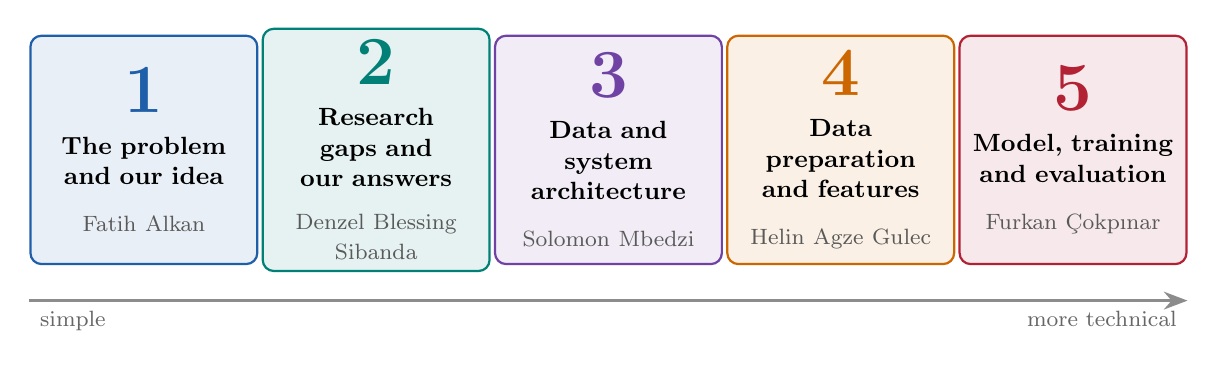
\begin{tikzpicture}[
  part/.style={rounded corners=4pt, text width=2.6cm, minimum height=2.9cm, align=center,
               inner sep=4pt, font=\small,
               execute at begin node={\hyphenpenalty=10000\exhyphenpenalty=10000}}]
  \foreach \n/\who/\topic in {
    1/Fatih Alkan/{The problem and our idea},
    2/{Denzel Blessing\\Sibanda}/{Research gaps and our answers},
    3/Solomon Mbedzi/{Data and system architecture},
    4/Helin Agze Gulec/{Data preparation and features},
    5/Furkan \c{C}okp{\i}nar/{Model, training and evaluation}}{
    \node[part, fill=p\n!10, draw=p\n, line width=0.8pt] (n\n) at ({(\n-1)*2.95},0)
      {{\color{p\n}\Huge\bfseries \n}\\[4pt]{\bfseries \topic}\\[6pt]{\footnotesize\color{black!65}\who}};
  }
  \draw[-{Stealth[length=3mm]}, line width=1.2pt, black!45]
    ([yshift=-0.45cm]n1.south west) -- ([yshift=-0.45cm]n5.south east)
    node[pos=0.0, below right, font=\footnotesize, text=black!60] {simple}
    node[pos=1.0, below left, font=\footnotesize, text=black!60] {more technical};
\end{tikzpicture}
\end{center}
\vspace{1mm}
\begin{center}\small
Main question of this section: \emph{How does our machine learning approach solve the gaps\\
we found in earlier research?}
\end{center}
\end{frame}

% ===============================================================
% PART 1 - Fatih Alkan - The problem and our idea
% ===============================================================
\presenter{p1}{1}{Fatih Alkan}

\begin{frame}{The problem}
\begin{columns}[T,onlytextwidth]
\column{0.53\textwidth}
\begin{itemize}
  \item In London, the police record about \textbf{23,000 injury road accidents} every year.
  \item Road safety teams have \textbf{limited time and money}.
  \item They need to know \textbf{where} and \textbf{when} accidents are most likely,
        so they can act \emph{before} they happen.
  \item Today this is often done with simple ``hotspot'' lists based only on past accidents.
\end{itemize}
\column{0.43\textwidth}
\begin{keybox}[title=Our question]
\large For a small area of the city and a 3-hour period, what is the
\textbf{probability} that at least one accident will happen?
\end{keybox}
\vspace{2mm}
\begin{softbox}\small
\textbf{Important rule:} we only use information that we already know
\emph{before} the 3-hour period starts.
\end{softbox}
\end{columns}
\end{frame}

\begin{frame}{Our idea in one picture}
\begin{center}
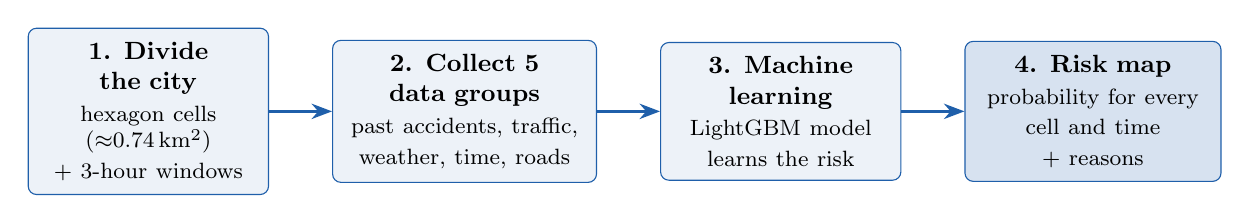
\begin{tikzpicture}[
  st/.style={rounded corners=3pt, align=center, font=\small, inner sep=5pt, minimum height=1.4cm},
  a/.style={-{Stealth[length=2.6mm]}, line width=1pt, p1}]
  % Step 1: grid
  \node[st, draw=p1, fill=p1!8, text width=2.7cm] (g) at (0,0)
    {\textbf{1. Divide the city}\\[2pt]\footnotesize hexagon cells\\($\approx$0.74\,km$^2$)\\+ 3-hour windows};
  % Step 2: data
  \node[st, draw=p1, fill=p1!8, text width=3.0cm, right=0.8cm of g] (d)
    {\textbf{2. Collect 5 data groups}\\[2pt]\footnotesize past accidents, traffic,\\weather, time, roads};
  % Step 3: model
  \node[st, draw=p1, fill=p1!8, text width=2.7cm, right=0.8cm of d] (m)
    {\textbf{3. Machine learning}\\[2pt]\footnotesize LightGBM model\\learns the risk};
  % Step 4: output
  \node[st, draw=p1, fill=p1!18, text width=2.9cm, right=0.8cm of m] (o)
    {\textbf{4. Risk map}\\[2pt]\footnotesize probability for every\\cell and time + reasons};
  \draw[a] (g) -- (d); \draw[a] (d) -- (m); \draw[a] (m) -- (o);
\end{tikzpicture}
\end{center}
\vspace{1mm}
\begin{columns}[T,onlytextwidth]
\column{0.48\textwidth}
\begin{softbox}\small
\textbf{What is new in our approach}\\[2pt]\footnotesize
\textcolor{p1}{$\blacksquare$} only free, open data\\
\textcolor{p1}{$\blacksquare$} real probabilities, not only rankings\\
\textcolor{p1}{$\blacksquare$} an explanation for every prediction
\end{softbox}
\column{0.48\textwidth}
\begin{softbox}\small
\textbf{Expected improvements} {\footnotesize(not yet tested)}\\[2pt]\footnotesize
\textcolor{p1}{$\blacksquare$} find more future accidents in top-risk areas\\
\textcolor{p1}{$\blacksquare$} more reliable and easier to trust\\
\textcolor{p1}{$\blacksquare$} can be repeated in other UK cities
\end{softbox}
\end{columns}
\end{frame}

% ===============================================================
% PART 2 - Denzel Blessing Sibanda - Gaps and answers
% ===============================================================
\presenter{p2}{2}{Denzel Blessing Sibanda}

\begin{frame}{What is missing in earlier research?}
\small
We reviewed statistical crash models and recent deep learning models
(e.g.\ Hetero-ConvLSTM, RiskOracle, GSNet). We found \textbf{six gaps}:
\vspace{2mm}
\begin{columns}[T,onlytextwidth]
\column{0.48\textwidth}
\begin{softbox}\textbf{\color{p2}G1 \ Wrong framing / leakage}\\\footnotesize
Many studies use only accident records, or data written \emph{after} the accident.
\end{softbox}
\begin{softbox}\textbf{\color{p2}G2 \ Too few factors}\\\footnotesize
Often only one or two data types; traffic volume is usually missing.
\end{softbox}
\begin{softbox}\textbf{\color{p2}G3 \ Accidents are rare}\\\footnotesize
Over 99\% of cases have no accident, so ``accuracy'' looks good even for bad models.
\end{softbox}
\column{0.48\textwidth}
\begin{softbox}\textbf{\color{p2}G4 \ Optimistic testing}\\\footnotesize
Random train/test splits let the model ``see the future''.
\end{softbox}
\begin{softbox}\textbf{\color{p2}G5 \ Black-box models}\\\footnotesize
Deep models do not explain \emph{why} an area is risky.
\end{softbox}
\begin{softbox}\textbf{\color{p2}G6 \ Untrusted numbers}\\\footnotesize
Scores are not real probabilities, and data or code are often private.
\end{softbox}
\end{columns}
\end{frame}

\begin{frame}{From each gap to our solution}
\footnotesize
\renewcommand{\arraystretch}{1.28}
\begin{tabularx}{\textwidth}{@{}>{\bfseries\color{p2}}l >{\raggedright\arraybackslash}X >{\raggedright\arraybackslash}X@{}}
\toprule
\color{ink}Gap & \textbf{Our solution} & \textbf{Expected result} \\
\midrule
G1 & Predict for \emph{every} cell and window; use only ``before'' information & Honest, realistic performance \\
G2 & Combine 5 open data groups, including traffic volume & Separate busy roads from dangerous roads \\
G3 & Keep all accidents, sample the rest, weighted loss; measure with PR-AUC and Recall@k & Find more real high-risk cases \\
G4 & Train on 2018--2022, tune on 2023, test once on 2024 & Results that hold for the future \\
G5 & SHAP explanations for every prediction & Road teams understand \emph{why} \\
G6 & Calibration of probabilities; open data and public code & ``5\% risk'' really means 5\%; others can repeat it \\
\bottomrule
\end{tabularx}
\vspace{2mm}
\begin{center}\scriptsize\color{black!60}
Every row is linked to a planned experiment (E1--E8), so each claim can be tested.
\end{center}
\end{frame}

% ===============================================================
% PART 3 - Solomon Mbedzi - Data and architecture
% ===============================================================
\presenter{p3}{3}{Solomon Mbedzi}

\begin{frame}{Our data: five open sources}
\begin{columns}[T,onlytextwidth]
\column{0.62\textwidth}
\footnotesize
\renewcommand{\arraystretch}{1.25}
\begin{tabularx}{\linewidth}{@{}>{\bfseries\color{p3}}l >{\raggedright\arraybackslash}X@{}}
\toprule
\color{ink}Data group & \textbf{Source and what we use} \\
\midrule
Past accidents & DfT STATS19: location, date, time of each accident \\
Traffic & DfT traffic counts (AADF) + hourly profile (TRA0307) \\
Weather & Open-Meteo: rain, temperature, wind, snow (hourly) \\
Time & hour, weekday, month, holidays, darkness \\
Roads & OpenStreetMap: road types, junctions, signals, crossings \\
\bottomrule
\end{tabularx}
\vspace{1mm}
{\scriptsize\color{black!60} All sources are free and openly licensed.}
\column{0.34\textwidth}\vspace{-1mm}
\begin{keybox}[title=Study design]
\small
\textbf{Area:} Greater London\\
\textbf{Cells:} $\approx$2,200 hexagons\\
\textbf{Time:} 3-hour windows\\
\textbf{Years:} 2018--2024\\
\textbf{Rows:} $\approx$6.4 million per year\\
\textbf{Accident rate:} only $\approx$0.3--0.4\%
\end{keybox}
\end{columns}
\vspace{0mm}
\begin{softbox}\small
\textbf{Target:} \;$y=1$ if at least one accident happens in the cell during the window, otherwise $y=0$.
\end{softbox}
\end{frame}

\begin{frame}{System architecture}
\vspace{-1mm}
\begin{center}
\resizebox{!}{0.66\textheight}{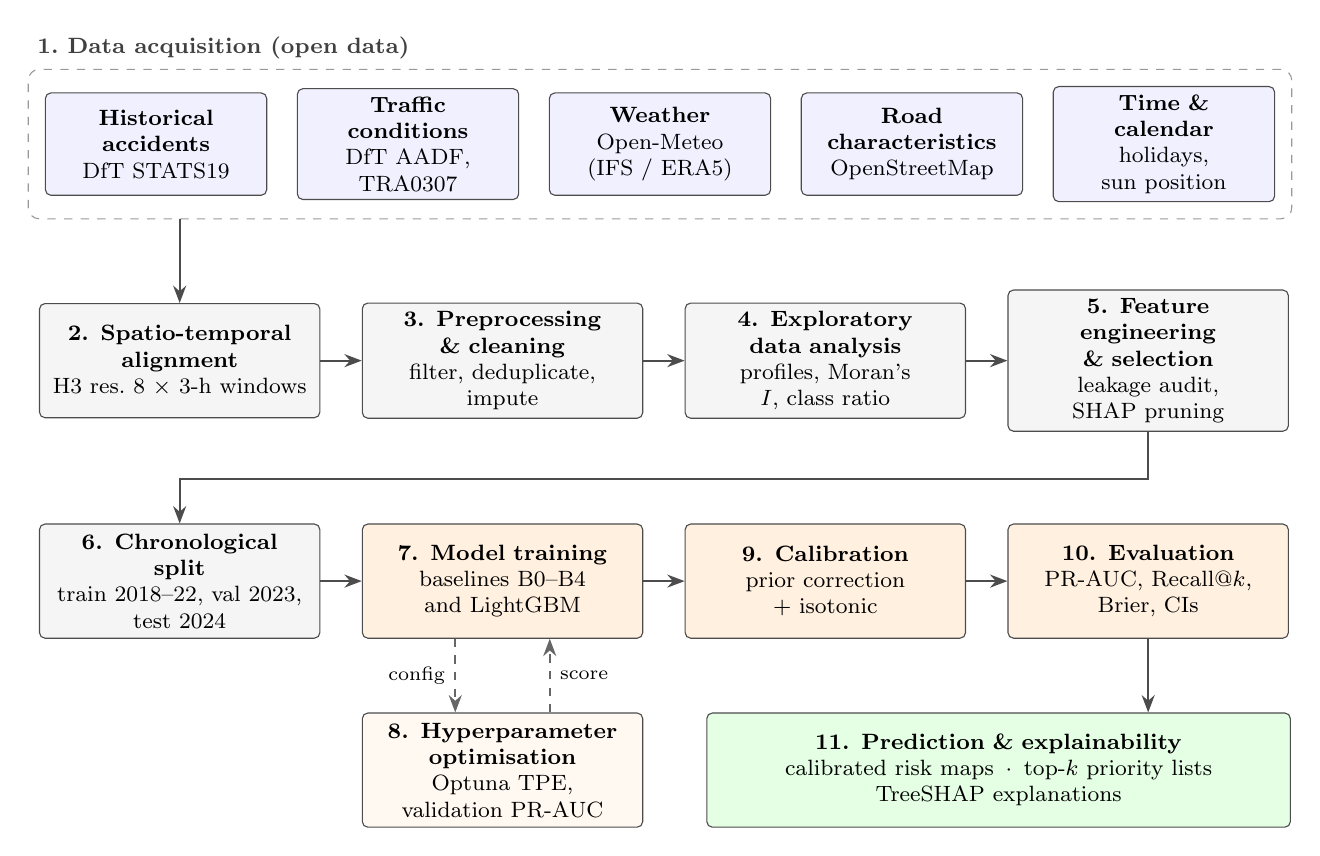
\begin{tikzpicture}[
  every node/.style={font=\footnotesize},
  sbox/.style={src, text width=2.6cm, minimum height=1.3cm},
  pbox/.style={proc, text width=3.35cm, minimum height=1.45cm},
  mbox/.style={model, text width=3.35cm, minimum height=1.45cm},
  obox/.style={resbox, text width=7.2cm, minimum height=1.45cm}
]
% ---- Data layer -------------------------------------------------
\node[sbox] (s1) at (1.40,0) {\textbf{Historical}\\\textbf{accidents}\\DfT STATS19};
\node[sbox] (s2) at (4.60,0) {\textbf{Traffic}\\\textbf{conditions}\\DfT AADF, TRA0307};
\node[sbox] (s3) at (7.80,0) {\textbf{Weather}\\Open-Meteo\\(IFS / ERA5)};
\node[sbox] (s4) at (11.00,0) {\textbf{Road}\\\textbf{characteristics}\\OpenStreetMap};
\node[sbox] (s5) at (14.20,0) {\textbf{Time \&}\\\textbf{calendar}\\holidays, sun position};
\begin{scope}[on background layer]
  \node[group, fit=(s1)(s5), inner ysep=6pt] (gA) {};
\end{scope}
\node[glabel, anchor=south west] at (gA.north west) {1.\ Data acquisition (open data)};

% ---- Preparation layer ------------------------------------------
\node[pbox] (b2) at (1.70,-2.75) {\textbf{2. Spatio-temporal}\\\textbf{alignment}\\H3 res.~8 $\times$ 3-h windows};
\node[pbox] (b3) at (5.80,-2.75) {\textbf{3. Preprocessing}\\\textbf{\& cleaning}\\filter, deduplicate, impute};
\node[pbox] (b4) at (9.90,-2.75) {\textbf{4. Exploratory}\\\textbf{data analysis}\\profiles, Moran's $I$, class ratio};
\node[pbox] (b5) at (14.00,-2.75) {\textbf{5. Feature engineering}\\\textbf{\& selection}\\leakage audit, SHAP pruning};

% ---- Modelling layer --------------------------------------------
\node[pbox] (c6) at (1.70,-5.55) {\textbf{6. Chronological}\\\textbf{split}\\train 2018--22, val 2023,\\test 2024};
\node[mbox] (c7) at (5.80,-5.55) {\textbf{7. Model training}\\baselines B0--B4\\and LightGBM};
\node[mbox] (c9) at (9.90,-5.55) {\textbf{9. Calibration}\\prior correction\\+ isotonic};
\node[mbox] (c10) at (14.00,-5.55) {\textbf{10. Evaluation}\\PR-AUC, Recall@$k$,\\Brier, CIs};

% ---- Optimisation and output ------------------------------------
\node[mbox, fill=orange!5] (d8) at (5.80,-7.95) {\textbf{8. Hyperparameter}\\\textbf{optimisation}\\Optuna TPE, validation PR-AUC};
\node[obox] (d11) at (12.10,-7.95) {\textbf{11. Prediction \& explainability}\\calibrated risk maps \,$\cdot$\, top-$k$ priority lists\\TreeSHAP explanations};

% ---- Arrows -----------------------------------------------------
\draw[arr] (gA.south -| b2.north) -- (b2.north);
\draw[arr] (b2) -- (b3);
\draw[arr] (b3) -- (b4);
\draw[arr] (b4) -- (b5);
\draw[arr] (b5.south) -- (b5.south |- 0,-4.25) -| (c6.north);
\draw[arr] (c6) -- (c7);
\draw[arr] (c7) -- (c9);
\draw[arr] (c9) -- (c10);
\draw[arr] (c10.south) -- (c10.south |- d11.north);
\draw[darr] ([xshift=-6mm]c7.south) -- ([xshift=-6mm]d8.north) node[midway, left, font=\scriptsize] {config};
\draw[darr] ([xshift=6mm]d8.north) -- ([xshift=6mm]c7.south) node[midway, right, font=\scriptsize] {score};
\end{tikzpicture}
}
\end{center}
\vspace{-4mm}
\begin{center}\scriptsize\color{black!65}
From raw data to risk maps in 11 steps. The dashed loop: the model is tuned on the validation year.
\end{center}
\end{frame}

% ===============================================================
% PART 4 - Helin Agze Gulec - Preparation and features
% ===============================================================
\presenter{p4}{4}{Helin Agze Gulec}

\begin{frame}{Preparing the data}
\vspace{-1mm}
\begin{columns}[T,onlytextwidth]
\column{0.67\textwidth}
\resizebox{\linewidth}{!}{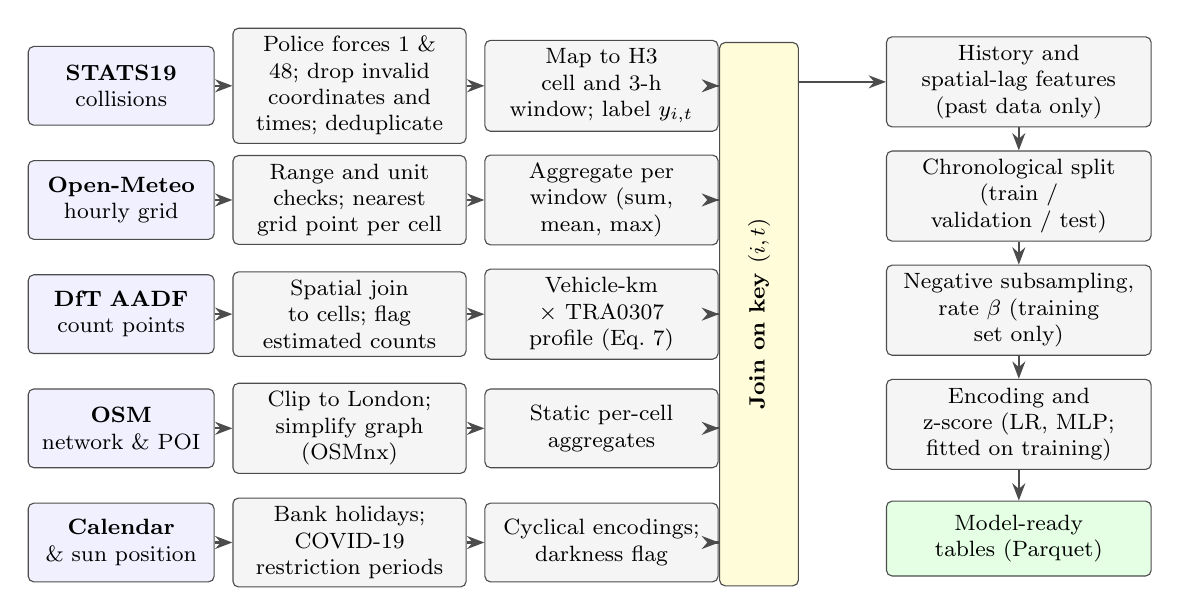
\begin{tikzpicture}[
  every node/.style={font=\footnotesize},
  sbox/.style={src, text width=2.15cm, minimum height=1.0cm},
  pbox/.style={proc, text width=2.75cm, minimum height=1.0cm},
  kbox/.style={proc, text width=3.15cm, minimum height=0.95cm}
]
% ---- Lanes: source -> cleaning -> aggregation ---------------------
\foreach \y/\s/\a/\b/\n in {
   0.0/{\textbf{STATS19}\\collisions}/{Police forces 1 \& 48; drop invalid coordinates and times; deduplicate}/{Map to H3 cell and 3-h window; label $y_{i,t}$}/L1,
  -1.45/{\textbf{Open-Meteo}\\hourly grid}/{Range and unit checks; nearest grid point per cell}/{Aggregate per window (sum, mean, max)}/L2,
  -2.90/{\textbf{DfT AADF}\\count points}/{Spatial join to cells; flag estimated counts}/{Vehicle-km $\times$ TRA0307 profile (Eq.~7)}/L3,
  -4.35/{\textbf{OSM}\\network \& POI}/{Clip to London; simplify graph (OSMnx)}/{Static per-cell aggregates}/L4,
  -5.80/{\textbf{Calendar}\\\& sun position}/{Bank holidays; COVID-19 restriction periods}/{Cyclical encodings; darkness flag}/L5}
{
  \node[sbox] (\n s) at (1.15,\y) {\s};
  \node[pbox] (\n a) at (4.05,\y) {\a};
  \node[pbox] (\n b) at (7.25,\y) {\b};
  \draw[arr] (\n s) -- (\n a);
  \draw[arr] (\n a) -- (\n b);
}

% ---- Join node spanning all lanes --------------------------------
\node[draw=black!70, rounded corners=2pt, fill=yellow!15, minimum width=1.0cm,
      fit={(9.25,0.55) (9.25,-6.35)}, inner sep=0pt] (join) {};
\node[rotate=90, font=\footnotesize\bfseries] at (join.center) {Join on key $(i,t)$};
\foreach \n in {L1,L2,L3,L4,L5}{
  \draw[arr] (\n b.east) -- (\n b.east -| join.west);
}

% ---- Post-join chain ---------------------------------------------
\node[kbox] (k1) at (12.55,0.05) {History and spatial-lag features (past data only)};
\node[kbox] (k2) at (12.55,-1.40) {Chronological split\\(train / validation / test)};
\node[kbox] (k3) at (12.55,-2.85) {Negative subsampling, rate $\beta$ (training set only)};
\node[kbox] (k4) at (12.55,-4.30) {Encoding and z-score (LR, MLP; fitted on training)};
\node[resbox, text width=3.15cm, minimum height=0.95cm] (k5) at (12.55,-5.75) {Model-ready tables (Parquet)};

\draw[arr] (join.east |- k1.west) -- (k1.west);
\draw[arr] (k1) -- (k2);
\draw[arr] (k2) -- (k3);
\draw[arr] (k3) -- (k4);
\draw[arr] (k4) -- (k5);
\end{tikzpicture}
}
\column{0.30\textwidth}
\begin{keybox}[title=Two golden rules]
\small
\textbf{1.} Features use \textbf{only the past}.\\[4pt]
\textbf{2.} Scalers and calibrators learn \textbf{only from training/validation years}.
\end{keybox}
\vspace{1mm}
\begin{softbox}\footnotesize
Police notes like ``wet road'' are written \emph{after} the accident, so we do \textbf{not} use them.
We use rain data and sun position instead.
\end{softbox}
\end{columns}
\end{frame}

\begin{frame}{Turning data into features}
\vspace{-3mm}
\begin{columns}[T,onlytextwidth]
\column{0.49\textwidth}
\begin{softbox}\footnotesize\textbf{Standardisation} (for linear model and MLP)
\eqline{z=\frac{x-\mu}{\sigma}}{3}
mean $\mu$ and std.\ $\sigma$ from training years only
\end{softbox}
\begin{softbox}\footnotesize\textbf{Cyclical time} (23:00 is close to 00:00)
\eqline{u_{\sin}=\sin\tfrac{2\pi u}{P},\;\; u_{\cos}=\cos\tfrac{2\pi u}{P}}{4}
$P=8$ windows per day, $P=12$ months
\end{softbox}
\begin{softbox}\footnotesize\textbf{Traffic exposure} (vehicle-km)
\eqline{E_{i,t}=\omega_{d,w}\textstyle\sum_{c\in\mathcal{C}_i} A_{c}\,L_{c}}{7}
$A$ daily traffic, $L$ road length, $\omega$ share in the window
\end{softbox}
\column{0.49\textwidth}
\begin{softbox}\footnotesize\textbf{Accident history} (recent accidents count more)
\eqline{h_{i,t}=\textstyle\sum_{\tau<t} e^{-(t-\tau)/\kappa}\,N_{i,\tau}}{5}
$N$ accidents in a past window, $\kappa$ decay speed
\end{softbox}
\begin{softbox}\footnotesize\textbf{Neighbour average} (spatial lag)
\eqline{s^{(k)}_{i,t}=\tfrac{1}{|\mathcal{R}_k(i)|}\textstyle\sum_{j\in\mathcal{R}_k(i)} h_{j,t}}{6}
average over the 6 (or 18) neighbour cells
\end{softbox}
\begin{keybox}
\footnotesize\textbf{Feature selection:} leakage check $\rightarrow$ remove constant features
$\rightarrow$ remove near-duplicates ($|\rho|>0.95$) $\rightarrow$ SHAP pruning
\end{keybox}
\end{columns}
\end{frame}

% ===============================================================
% PART 5 - Furkan Cokpinar - Model, training and evaluation
% ===============================================================
\presenter{p5}{5}{Furkan \c{C}okp{\i}nar}

\begin{frame}{The model: LightGBM with calibration}
\vspace{-3mm}
\begin{center}
\resizebox{0.74\linewidth}{!}{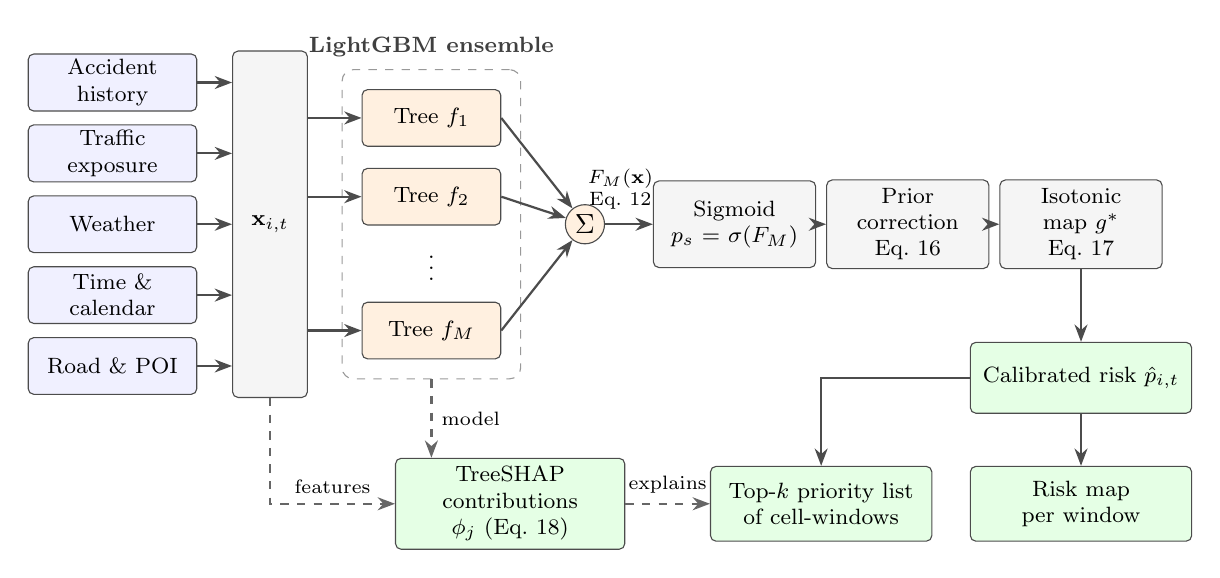
\begin{tikzpicture}[
  every node/.style={font=\footnotesize},
  fbox/.style={src, text width=2.0cm, minimum height=0.72cm, inner sep=2pt},
  tbox/.style={model, text width=1.55cm, minimum height=0.72cm},
  cbox/.style={proc, text width=1.85cm, minimum height=1.1cm}
]
% ---- Feature groups ----------------------------------------------
\node[fbox] (f1) at (1.05, 1.80) {Accident history};
\node[fbox] (f2) at (1.05, 0.90) {Traffic exposure};
\node[fbox] (f3) at (1.05, 0.00) {Weather};
\node[fbox] (f4) at (1.05,-0.90) {Time \& calendar};
\node[fbox] (f5) at (1.05,-1.80) {Road \& POI};

% ---- Feature vector ----------------------------------------------
\node[draw=black!70, rounded corners=2pt, fill=gray!8, minimum width=0.95cm,
      fit={(3.05,2.2) (3.05,-2.2)}, inner sep=0pt] (xv) {};
\node at (xv.center) {$\mathbf{x}_{i,t}$};
\foreach \n in {f1,f2,f3,f4,f5}{ \draw[arr] (\n.east) -- (\n.east -| xv.west); }

% ---- Boosted trees -----------------------------------------------
\node[tbox] (t1) at (5.10, 1.35) {Tree $f_1$};
\node[tbox] (t2) at (5.10, 0.35) {Tree $f_2$};
\node       (td) at (5.10,-0.45) {$\vdots$};
\node[tbox] (tm) at (5.10,-1.35) {Tree $f_M$};
\begin{scope}[on background layer]
  \node[group, fit=(t1)(tm), inner sep=7pt] (ens) {};
\end{scope}
\node[glabel, anchor=south, yshift=1pt] at (ens.north) {LightGBM ensemble};
\foreach \n in {t1,t2,tm}{ \draw[arr] (xv.east |- \n.west) -- (\n.west); }

% ---- Sum node ----------------------------------------------------
\node[circle, draw=black!70, fill=orange!12, inner sep=1.5pt, font=\normalsize] (sum) at (7.05,0) {$\Sigma$};
\foreach \n in {t1,t2,tm}{ \draw[arr] (\n.east) -- (sum); }
\node[font=\scriptsize, align=center, anchor=south] at (7.5,0.06) {$F_M(\mathbf{x})$\\Eq.~12};

% ---- Probability and calibration chain ---------------------------
\node[cbox] (sig) at (8.95,0) {Sigmoid\\$p_s=\sigma(F_M)$};
\node[cbox] (pc)  at (11.15,0) {Prior correction\\Eq.~16};
\node[cbox] (iso) at (13.35,0) {Isotonic map $g^{*}$\\Eq.~17};
\draw[arr] (sum) -- (sig);
\draw[arr] (sig) -- (pc);
\draw[arr] (pc) -- (iso);

\node[resbox, text width=2.6cm, minimum height=0.9cm] (p) at (13.35,-1.95) {Calibrated risk $\hat{p}_{i,t}$};
\draw[arr] (iso) -- (p);

% ---- Outputs -----------------------------------------------------
\node[resbox, text width=2.7cm, minimum height=0.95cm] (o1) at (6.10,-3.55) {TreeSHAP contributions $\phi_j$ (Eq.~18)};
\node[resbox, text width=2.6cm, minimum height=0.95cm] (o2) at (10.05,-3.55) {Top-$k$ priority list of cell-windows};
\node[resbox, text width=2.6cm, minimum height=0.95cm] (o3) at (13.35,-3.55) {Risk map per window};

\draw[arr] (p.south) -- (o3.north);
\draw[arr] (p.west) -| (o2.north);
\draw[darr] (ens.south) -- (ens.south |- o1.north) node[midway, right, font=\scriptsize] {model};
\draw[darr] (xv.south) |- (o1.west) node[pos=0.75, above, font=\scriptsize] {features};
\draw[darr] (o1.east) -- (o2.west) node[midway, above, font=\scriptsize] {explains};
\end{tikzpicture}
}
\end{center}
\vspace{-3mm}
\begin{softbox}\scriptsize
\begin{tabularx}{\linewidth}{@{}>{\hsize=0.85\hsize}X >{\hsize=1.35\hsize}X >{\hsize=0.8\hsize}X@{}}
\textbf{Many small trees}\hfill{\color{black!55}(12)} &
\textbf{Weighted loss}\hfill{\color{black!55}(10)} &
\textbf{Undo the sampling}\hfill{\color{black!55}(16)} \\[4pt]
\centering $F_M(\mathbf{x})=F_0+\eta\sum_{m=1}^{M} f_m(\mathbf{x})$ &
\centering $\mathcal{L}=-\frac{1}{n}\sum\big[w_{+}y\log\hat p+(1-y)\log(1-\hat p)\big]$ &
\centering\arraybackslash $\hat p=\dfrac{\beta\,p_s}{\beta\,p_s+1-p_s}$
\end{tabularx}
\end{softbox}
\end{frame}

\begin{frame}{Training and evaluation}
\vspace{-2mm}
\begin{center}
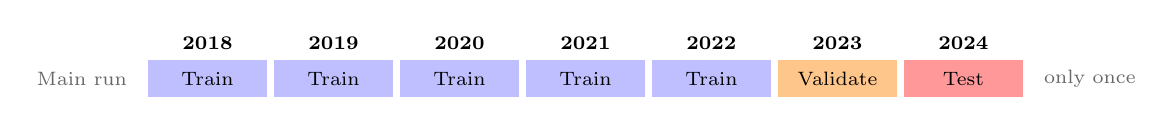
\begin{tikzpicture}[yr/.style={minimum width=1.55cm, minimum height=0.5cm, inner sep=0pt,
                     font=\scriptsize, draw=white, line width=1pt}]
  \foreach \k/\y in {0/2018,1/2019,2/2020,3/2021,4/2022,5/2023,6/2024}{
    \node[font=\scriptsize\bfseries] at (\k*1.6,0.45) {\y};
  }
  \foreach \k in {0,...,4}{ \node[yr, fill=blue!25] at (\k*1.6,0) {Train}; }
  \node[yr, fill=orange!45] at (5*1.6,0) {Validate};
  \node[yr, fill=red!40] at (6*1.6,0) {Test};
  \node[anchor=east, font=\scriptsize, text=black!60] at (-0.9,0) {Main run};
  \node[anchor=west, font=\scriptsize, text=black!60] at (6*1.6+0.9,0) {only once};
\end{tikzpicture}
\end{center}
\vspace{-1mm}
\begin{columns}[T,onlytextwidth]
\column{0.52\textwidth}
\begin{softbox}\scriptsize
\textbf{How we measure} (accuracy is useless: ``no accident'' is right 99.6\% of the time)
\vspace{-2mm}
\begin{align*}
\text{Precision}&=\tfrac{TP}{TP+FP}, \quad \text{Recall}=\tfrac{TP}{TP+FN} \tag*{\color{black!55}(19--20)}\\
\text{F1}&=2\cdot\tfrac{\text{Precision}\cdot\text{Recall}}{\text{Precision}+\text{Recall}} \tag*{\color{black!55}(21)}\\
\text{Recall@}k&=\tfrac{\text{accidents in top }k\%}{\text{all accidents}} \tag*{\color{black!55}(24)}\\
\text{Brier}&=\tfrac{1}{n}\textstyle\sum(\hat p-y)^2 \tag*{\color{black!55}(25)}
\end{align*}
\vspace{-6mm}\\
\textbf{Main metric:} PR-AUC (good for rare events).
\end{softbox}
\column{0.45\textwidth}
\begin{keybox}[title=We compare with]
\scriptsize
B0 historical rate \;\textbullet\; B1 logistic regression\\
B2 random forest \;\textbullet\; B3 neural network (MLP)\\
B4 XGBoost \;\textbullet\; \textbf{LightGBM (ours)}
\end{keybox}
\vspace{-1mm}
\begin{softbox}\scriptsize
\textbf{Tuning:} Optuna, 100 trials, early stopping\\
\textbf{Fair test:} 95\% confidence intervals with block bootstrap\\
\textbf{Limits:} yearly traffic data, $\approx$10\,km weather grid, only police-reported accidents
\end{softbox}
\end{columns}
\end{frame}

% ===============================================================
% Closing
% ===============================================================
\presenter{p1}{0}{}
\begin{frame}{Summary}
\begin{columns}[T,onlytextwidth]
\column{0.56\textwidth}
\begin{itemize}
  \item We predict the \textbf{probability of an accident} for every small area of London
        and every 3-hour period.
  \item Our solution answers all \textbf{six gaps} (G1--G6) from the literature.
  \item We use \textbf{open data}, a \textbf{LightGBM} model, \textbf{calibrated} probabilities
        and \textbf{SHAP} explanations.
  \item We test on a \textbf{future year} (2024), so our results will be realistic.
\end{itemize}
\column{0.40\textwidth}
\begin{keybox}[title=Next steps]
\small
1.\ Download and clean the data\\
2.\ Build the features\\
3.\ Train and tune the models\\
4.\ Run experiments E1--E8\\
5.\ Write results in the paper
\end{keybox}
\end{columns}
\vspace{4mm}
\begin{center}
{\Large\bfseries Thank you! \ Questions?}\\[4pt]
{\scriptsize\color{black!60} Code, paper and plan: github.com/FatihAlkan79731/Machine-Learning-Team-Project}
\end{center}
\end{frame}

\end{document}
